
%%% Preamble
\documentclass[paper=a4,fontsize=11pt]{report}


%%% Begin document
\begin{document}

\title{
	%\vspace{-1in}
	\usefont{OT1}{bch}{b}{n}
	\normalfont \normalsize \textsc{Instituto Tecnológico de Buenos Aires} \\ [25pt]
	\horrule{2pt} \\[0.4cm]
	\huge Assignment $N^o 2$ \\
	\horrule{2pt} \\[0cm]
\author{Group 2:\\Díaz Ian Cruz\\Lin Benjamín\\ Müller Malena\\Oh Victor \\ \\ Professors:\\Dewald Kevin\\Wundus Pablo Enrique\\ \\}
\text{Electrónica 3 - 2018}
}
\date{\today} %ver si dejar la de today o poner fecha fija que sea August 2018
\pagenumbering{arabic}

\maketitle
\newpage

% The \input command appends the content of the file directly into the document.
%AGREGAR:
%fotos, graficos
%explicar y mostrar simulaciones
%comparar para el noise margin la simulacion con las distintas R
%lo del capacitor de 1 nF

\documentclass[a4paper,11pt]{report}

%\usepackage[options]{package}
\usepackage{graphicx}
\usepackage{color} 
\usepackage[dvipsnames]{xcolor}
\colorlet{purple}{purple}

\begin{document}

\section{\color{olive}Exercise 1: Design and Implementation of NOT Gates Using Transistors} %Despues borrar el Exercise 1 del titulo y que queden solo los titulos de los ejs en color olive.


\subsubsection{\color{red}High-Level and Low-Level Input Voltages}
The high-level input voltage ($V_{IH}$) is the minimum input voltage that is considered as high, while the low-level input voltage ($V_{IL}$)  is the maximum input voltage that is considered as low.

\subsubsection{\color{red}High-Level and Low-Level Output Voltages}
The high-level output voltage ($V_{OH}$) is the minimum output voltage that the circuit provides as a high, while the low-level output voltage ($V_{OL}$) is the maximum output voltage that the circuit provides as a low.

\subsubsection{\color{red}Noise Margin}
The high noise margin ($NM_{H}$) is the gap between the high-level input voltage and the high-level output voltage, while the low noise margin ($NM_{L}$) is the gap between the low-level output voltage and the low-level input voltage.
$$NM_{H} = V_{OH} - V_{IH}$$
$$NM_{L} = V_{IL} - V_{OL}$$

\subsubsection{\color{red}Propagation Delays}
For this assignment's meassures, when the input changes from low to hight and the output from high to low, the high-to-low propagation delay is considered as the time between the moment in which the input voltage reaches the $90\% $ of its maximum high value, until the moment in which the output voltage reaches the $10\%$ of its maximum high value.
$$t_{pHL} = t_{10\%V_{maxO}} - t_{90\%V_{maxI}}$$
In the case in which the input goes from high to low and the output from low to high, the low-to-high propagation delay is considered as the time between the moment in which the input voltage reaches the $10\%$ of its maximum high value, until the moment in which the output voltage reaches the $90\%$ of its maximum high value.
$$t_{pLH} = t_{90\%V_{maxO}} - t_{10\%V_{maxI}}$$

\subsubsection{\color{red}Transition Times}
The high-to-low transition time or fall time ($t_{f}$) is the time that it takes the output voltage to go from its high maximum value to its low minimum value, while the low-to-high transition time or rise time ($t_{r}$) is the time that it takes for it to change from its low minimum value to tis high maximum value.


\subsubsection{\color{red}Maximum Output Current}
%ESCRIBIR ACA LO DE LA DERIVADA DE LA TENSION EN EL OSCILOSCOPIO

\subsection{\color{purple}Measurements}


\subsection{\color{purple}Using a BJT NPN 337 Transistor}

\subsubsection{\color{red}Without Load Connected to the Output}

\subsubsection{\color{red}With a $1 nF$ Capacitor Connected to the Output}


\subsection{\color{purple}Using a BJT PNP 327 Transistor}

\subsubsection{\color{red}Without Load Connected to the Output}


\begin{tabular}{|c|c|c|c|c|}
\hline
 & NPN & NPN with capacitor &PNP& PNP with capacitor\\
\hline
\hline
$V_{IH} (V)$ & 0,9 & 0,9 & 4,5 & 4,6  \\
\hline
$V_{IL} (V)$ & 0,5V & 0,6 & 4,2 & 4,3 \\
\hline
$V_{OH} (V)$ & 4,96V & 4,56 & 4,77 & 5 \\
\hline
$V_{OL} (V)$ & 0,1 & 0,12 & 0,05 & 0,45\\ 
\hline
$NM_{H} (V) $ & 4,06 & 3,66 & 0,27 & 0,4\\ %se pone en VOLTS???????????????????????????
\hline
$NM_{L} (V) $ & 0,4 & 0,48 & 4,15 & 3,85 \\  %se pone en VOLTS???????????????????????????
\hline
$t_{pHL}$ & 87ns & $2,7\mu s $ &  $2,72\mu s$ & 101ns \\
\hline
$t_{pLH}$ & $2,94\mu s$ &  104ns &  73ns &  $2,23\mu s$\\
\hline
$t_{f}$ & 69,5ns & 84ns & 575ns & 770ns\\
\hline
$t_{r}$ & 505ns & 520ns & 83ns & 86 ns\\
\hline
$ I_{Out{Max}}$ &   &   &   &   \\ %AGREGAAAAAAAAAAAAAAAAAAAR
\hline
\end{tabular}

\end{document} 

























\input{../Exercise2/EX2.tex}
\section{\color{olive}Exercise 3: Simplification and Implementation of a Truth Table }

In this section, we will show how using the lower cost technology
to implement a truth table, can result in some glitches and issues.
For this exercise, we were asked to simplify the truth Table on Table
\ref{3_1}

\begin{table}[h!]
\begin{centering}
\begin{tabular}{|c|c|c|c|}
\hline 
A & B & C & O\tabularnewline
\hline 
\hline 
0 & 0 & 0 & 0\tabularnewline
\hline 
0 & 0 & 1 & 1\tabularnewline
\hline 
0 & 1 & 0 & 1\tabularnewline
\hline 
0 & 1 & 1 & 1\tabularnewline
\hline 
1 & 0 & 0 & 0\tabularnewline
\hline 
1 & 0 & 1 & 1\tabularnewline
\hline 
1 & 1 & 0 & 0\tabularnewline
\hline 
1 & 1 & 1 & 0\tabularnewline
\hline 
\end{tabular}
\par\end{centering}
\caption{\color{cyan}Truth Table}
\label{3_1}

\end{table}

When we express this in the form of the Karnaugh map, we'va got the
Figure \ref{3_2}. As we see there, if we do not take into account
the yellow minterm, there are two separate subsets of ones that can
represent the Table \ref{3_1}. However, as we know, because the two
subsets have no element in common, representing this truth tables
with just two minterms can cause glitches.

\begin{figure}[h!]
\begin{centering}
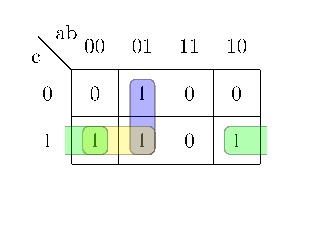
\includegraphics[scale=0.2]{../Exercise3/images/Karnaugh}
\par\end{centering}
\caption{\color{cyan}Karnaugh's Map}
\label{3_2}

\end{figure}

By implementing this wit NAND gates we've got the circuit shown on
Figure \ref{3_3}.

\begin{figure}[h!]
\begin{centering}
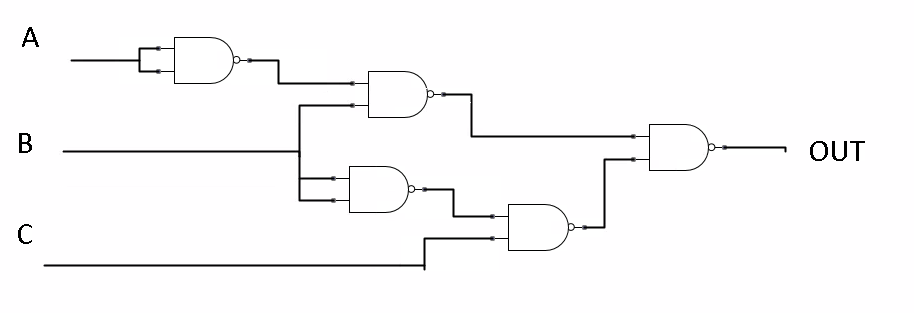
\includegraphics[scale=0.3]{../Exercise3/images/CIRCUIT}
\par\end{centering}
\caption{\color{cyan}NAND Circuit Implementation}
\label{3_3}

\end{figure}

Finally, when we tried to test the circuit shown, we noticed some
glitches of time less than 10 micorseconds, thes glitches are shown
on Figure \ref{3_4}.

\begin{figure}[h!]
\begin{centering}
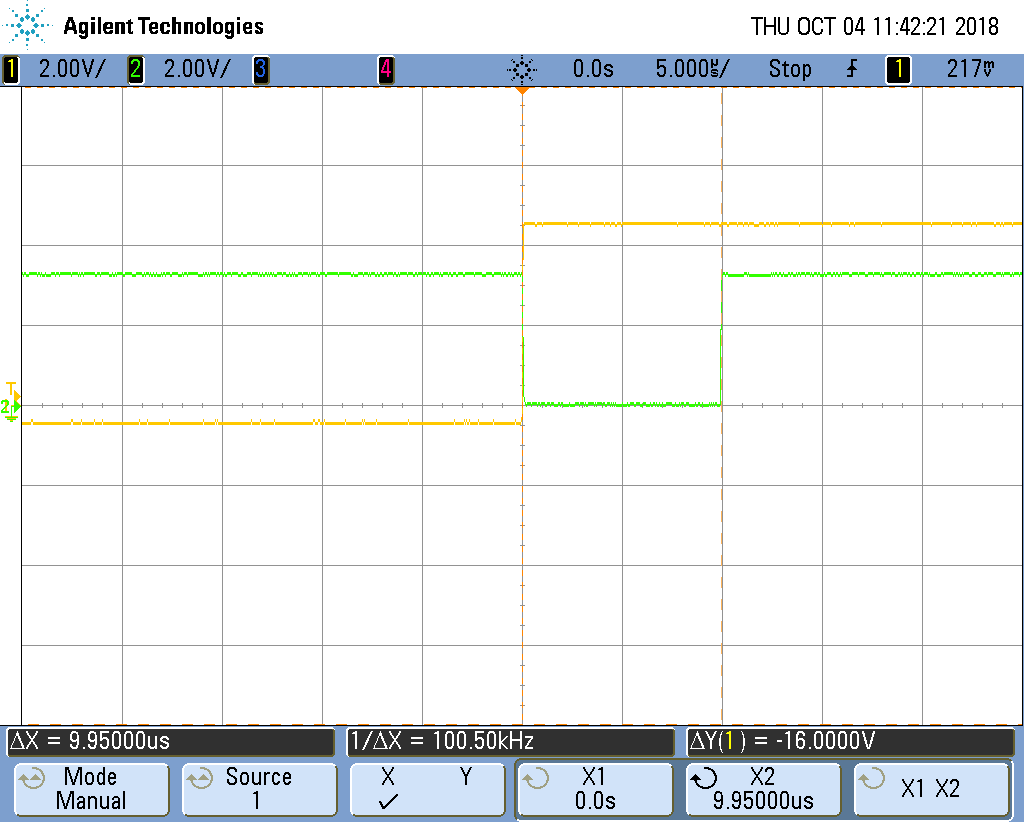
\includegraphics[scale=0.2]{../Exercise3/images/e3}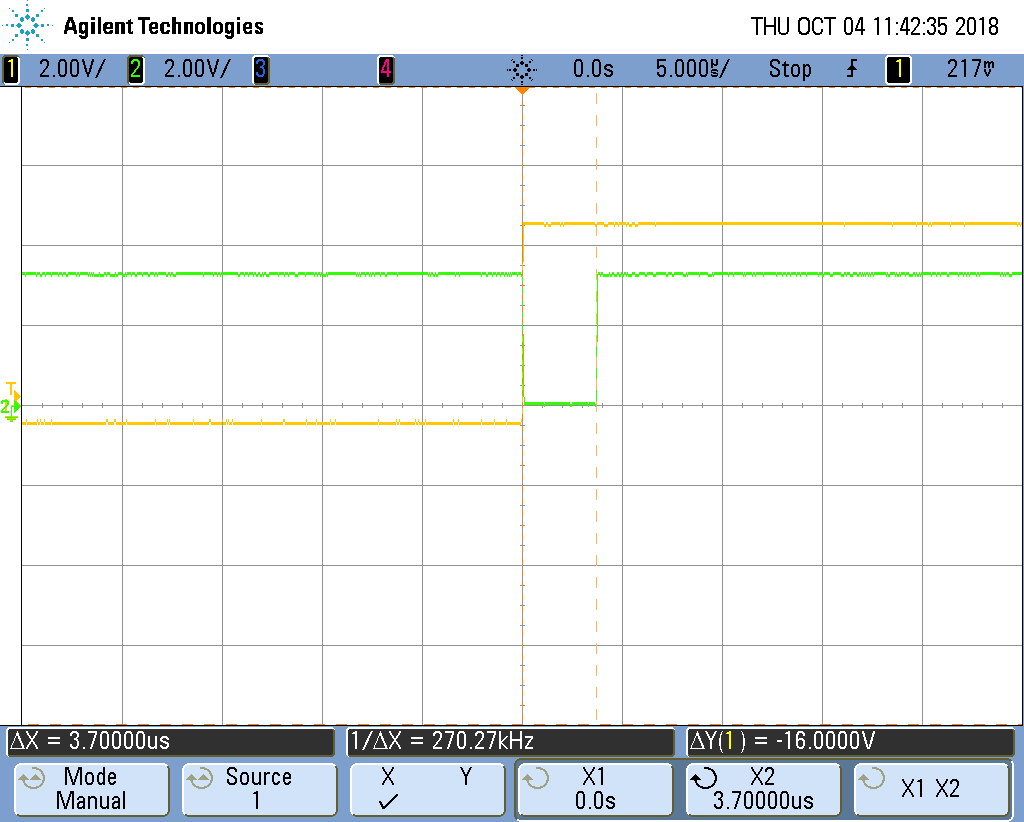
\includegraphics[scale=0.2]{../Exercise3/images/e4}
\par\end{centering}
\caption{\color{cyan}Glitches}
\label{3_4}

\end{figure}

This little negative peaks shouldn't be there since we were changing
from one positive state, to another positive state in both cases.
To resolve this, we only need to add a third minterm to the equation,
and this would be the yellow minterm on Figure \ref{3_2}.

\documentclass[a4paper,11pt]{report}

%\usepackage[options]{package}
\usepackage{graphicx}
\usepackage{color} 
\usepackage[dvipsnames]{xcolor}
\colorlet{purple}{purple}

\begin{document}


\section{\color{olive}Exercise 4: Behaviour Analysis of Circuits Including a 74HC02 Gate}

The 74HC02 is an integrated circuit of NOR gates. Firstly, the propagation delays and the transition times are measured for this gate in a no-load output condition. Then these parameters are measured in the case in which the gate is connected in the circuit in Figure. %HACER REFERENCIA A LA FOTITO
In the following table, the results of the mentioned measures are shown.
 %PONER FOTITO DE LA NOR (no load)
%foto circuito
%foto circuito con capacitor

\subsubsection{\color{red}Propagation and Transition Times' Measurements}

\begin{tabular}{|c|c|c|}
%\label{first meas}
\hline
 &No-load & Loaded with circuit \\ %aclarar haciendo referencia a la foto del circuito
\hline
\hline
$t_{pHL}$ & 1,5ns & 1,05ns \\
\hline
$t_{pLH}$ & 12,5ns & 14,4ns\\
\hline
$t_{f}$ & 32ns & 30,7ns\\
\hline
$t_{r}$ & 41,4ns & 43,2ns \\
\hline
\end{tabular}\\



In the previous table it can be seen that the four parameters remain practically the same while being the 74HC02 in the no-load situation and incorporated in the circuit. However, the small differences have opposite behaviours depending on the input signal's edge. In the case of a rising edge in the input signal, the propagation delay $t_{pLH}$ and the transition time $t_{r}$ are bigger if the 74HC02 forms part of the circuit, than if the 74HC02 is in a no-load situation. But the opposite occurs with the falling edge of the input. The propagation delay $t_{pHL}$ and the transition time $t_{f}$ are smaller when the 74HC00 forms part of the circuit in comparisson to when the no-load situation.

\subsubsection{\color{red}Circuit's Response to Frequency Increment}

No significable temperature changes were noticed in the integrated circuits nor in any component of the entire circuit.
The power discipated by the integrated circuit depends of $f^{2}$, and therefore, a temperature augmentation should be perceived by increasing the frequency from 1Hz to 100kHz. However, no significable temperature changes were noticed in the integrated circuits nor in any component of the entire circuit. Only a small temperature increase was perceived.
%buscar info de que depende la potencia discipada y hablar de eso 
% buscar formula de la potencia discipada por un chip. y ver de que parametros depende y de que forma.


\subsubsection{\color{red}Alimentation Voltage and Temperature of the IC}

It is seen in the osciloscope that the alimentation voltage of the circuit in Figure %AGREGAR REFERENCIA
has a ripple when there is an edge of the square input signal. This is due to the big ammount of current that the integrated circuit of NOR gates demands from the voltage source when the input signal rises from 0V to 5V or when it falls from 5V to 0V. 
In order to reduce this "ripple-shape" response of the circuits to such edges, a capacitor has to be added between the +Vcc and the GND terminals of the integrated circuit. The goal is to add a capacitor in a way that the less inductance is added to the circuit. This capacitor has to be the nearest possible to such terminals, to avoid adding long wires that add inductance. Moreover,  the best capacitors' technology for this case is the multilayer capacitor as it doesn't add as much inductance as other types of capacitors. As it is preffered to use a multilayer capacitor between 10nF and 100nF for this situation, we decided to use a 100nF capacitor and the ripple decreased, as it can be seen in Figure %AGREGAR REF (usar palabra desacople en ingles)


\end{document} 
%%%% Preamble
\documentclass[paper=a4,fontsize=11pt]{report}


%\begin{document}

%\begin{titlepage}
    
\newcommand{\HRule}{\rule{\linewidth}{0.5mm}} % Defines a new command for the horizontal lines, change thickness here
    
\center % Center everything on the page
     
%----------------------------------------------------------------------------------------
%	HEADING SECTIONS
%----------------------------------------------------------------------------------------
    
\textsc{\LARGE Instituto Tecnológico de Buenos Aires}\\[2cm] % Name of your university/college
\textsc{\Large Electronica III}\\[1.5cm] % Major heading such as course name
\textsc{\large Trabajo Práctico N° 2}\\[0.5cm] % Minor heading such as course title
    
%----------------------------------------------------------------------------------------
%	TITLE SECTION
%----------------------------------------------------------------------------------------
    
\HRule \\[0.5cm]
{ \huge \bfseries Trabajo Práctico de Laboratorio Nr. 2}\\[0.4cm] % Title of your document
\HRule \\[2cm]
     
%----------------------------------------------------------------------------------------
%	AUTHOR SECTION
%----------------------------------------------------------------------------------------
    
\begin{minipage}{0.4\textwidth}
\begin{flushleft} \large
\emph{Grupo 2:}\\		%names
[.3cm]
Victor \textsc{Oh}\\
Leg. ???\\ 
[.3cm]
Ian \textsc{Diaz}\\
Leg. ???\\ 
[.3cm]
Benjamín Carlos \textsc{Lin}\\
Leg. 57242 \\ 
[.3cm]
Malena \textsc{Muller}\\
Leg. ???\\ 
[.3cm]
\end{flushleft}
\end{minipage}
~
\begin{minipage}{0.4\textwidth}
\begin{flushright} \large
%\emph{Profesor:} \\
%[.3cm]
%Pablo  \textsc{Cossutta}\\ % Supervisor's Name
%Alejandra \textsc{Weill} \\% Supervisor's Name
%Matías  \textsc{Salvati} % Supervisor's Name
\end{flushright}
\end{minipage}\\[2cm]
    
%----------------------------------------------------------------------------------------
%	DATE SECTION
%----------------------------------------------------------------------------------------
    
\vfill
{\large Entregado: 17 de Octubre de 2018}\\[2cm]
    
\vfill 
    
\end{titlepage}
%
%\pagenumbering{roman}
%\tableofcontents
%\newpage
%\pagenumbering{arabic}
%
%Test Text

\section{\color{olive}Exercise 5: Compatibility between TTL and CMOS}

\subsection{\color{purple}Floating input in TTL and CMOS}

Connecting the following circuit in figure \ref{fig:ej5ttl} and \ref{fig:ej5cmos} leaving one of the inputs floating having $Vcc = 5V$. 

\begin{figure}[h!]
         \begin{minipage}{.47\linewidth}
        \centering
        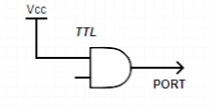
\includegraphics[width=.6\linewidth]{../Exercise5/TTL5.png}
        \caption{\color{cyan}Floating TTL}
        \label{fig:ej5ttl}
        \end{minipage}
         \begin{minipage}{.5\linewidth}
        \centering
        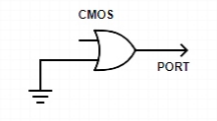
\includegraphics[width=.5\linewidth]{../Exercise5/CMOS5.png}
        \caption{\color{cyan}Floating CMOS}
        \label{fig:ej5cmos}
    \end{minipage}
\end{figure}

For the 74LS08, the TTL component, the output port value shown was a logical 1 constantly. On the other hand, the 74HC32, the CMOS component, the results were random with a frequency of 50Hz, having a quadratic function from 0 to 5V or 3 to 5V or a 0 to 0.8V amplitude function.

\begin{figure}[h!]
        \centering
        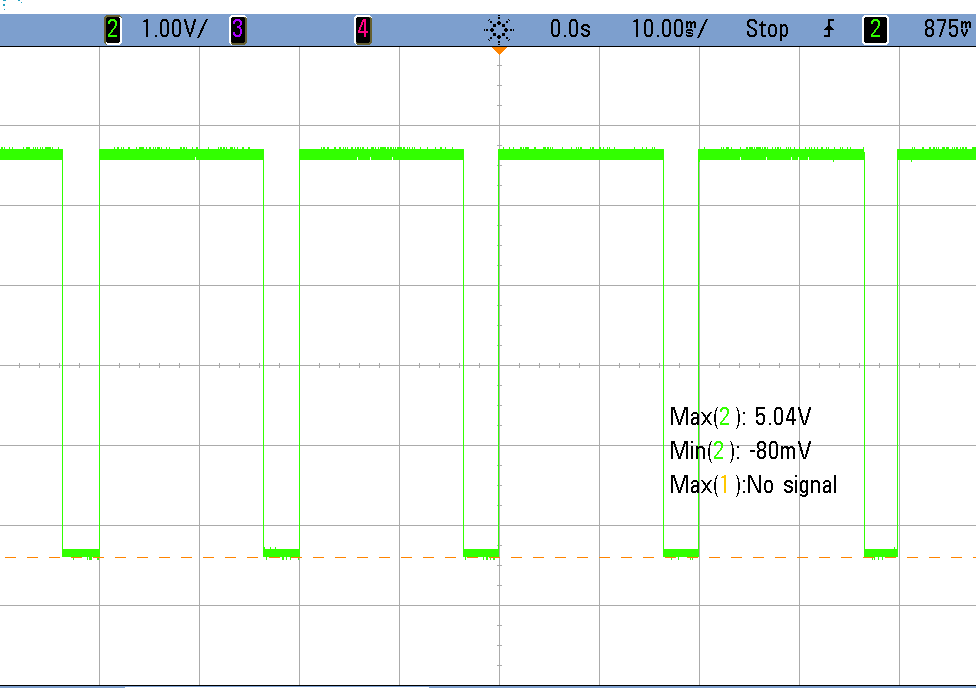
\includegraphics[scale=0.19]{../Exercise5/cmos_cerda2.png}\hspace{1cm}
%        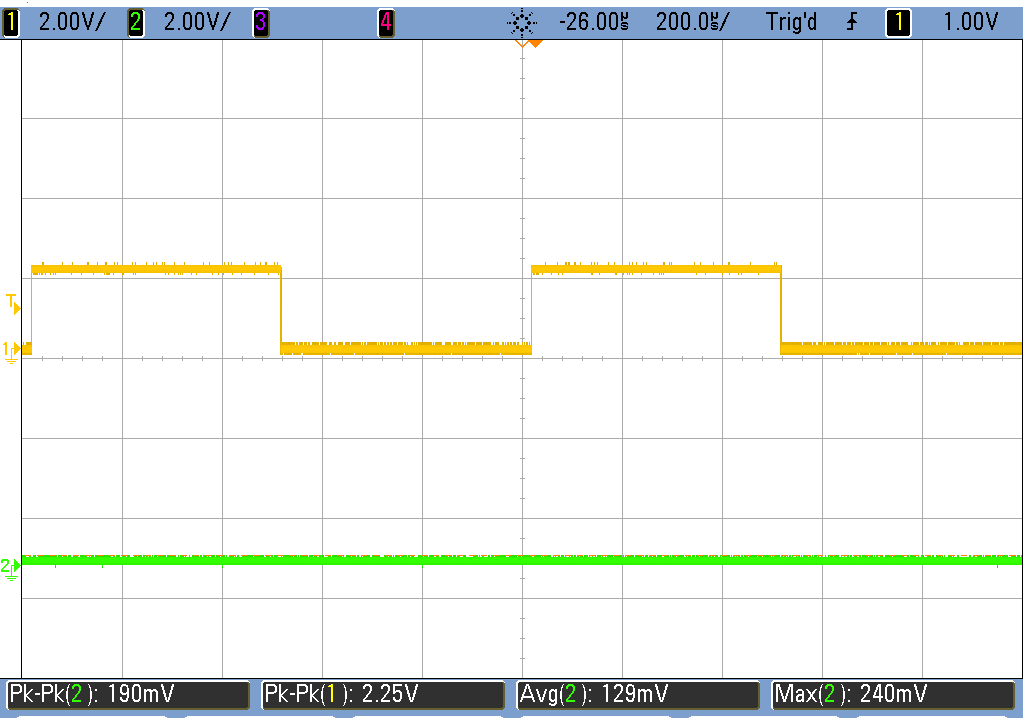
\includegraphics[scale=0.19]{HC-LS-2V.png}\\
        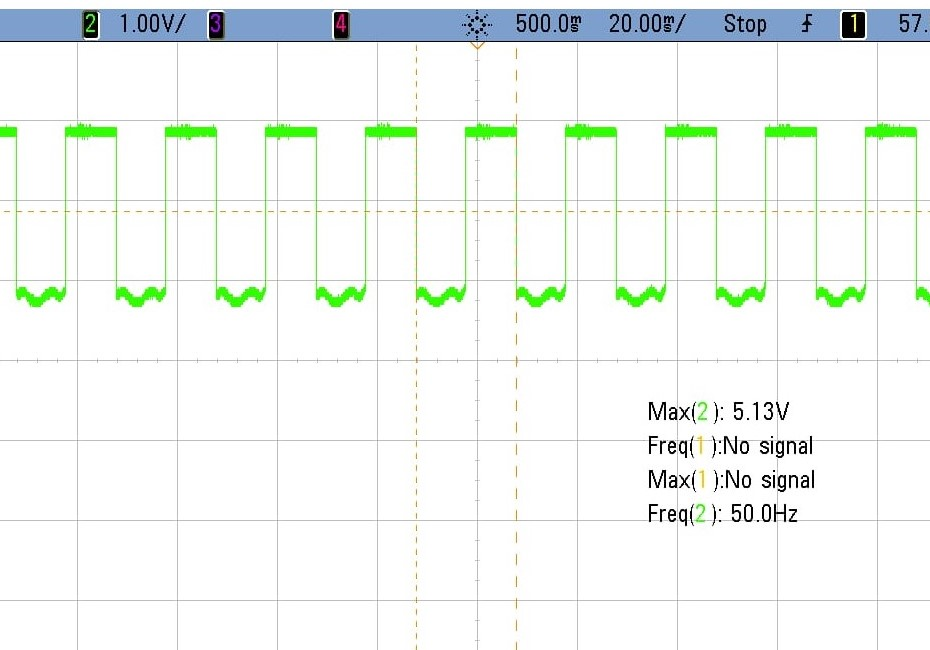
\includegraphics[scale=0.2]{../Exercise5/cmos_dads.jpeg}\\
		\vspace{0.2cm}
%		\hspace{0.9cm}
	   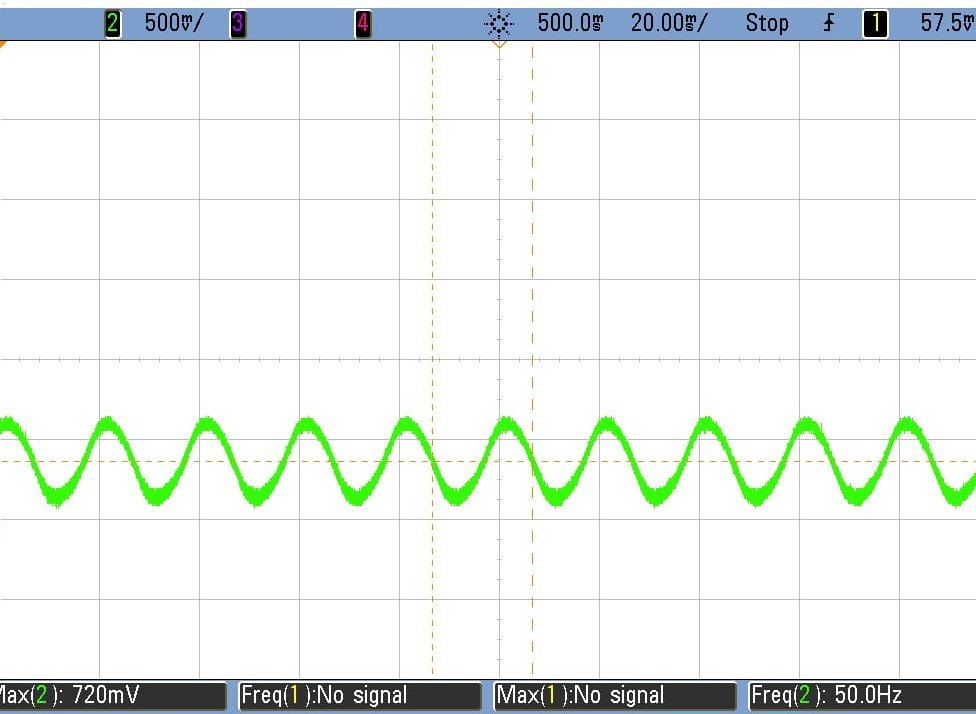
\includegraphics[scale=0.19]{../Exercise5/cmos_ahifdas.jpeg} 
%        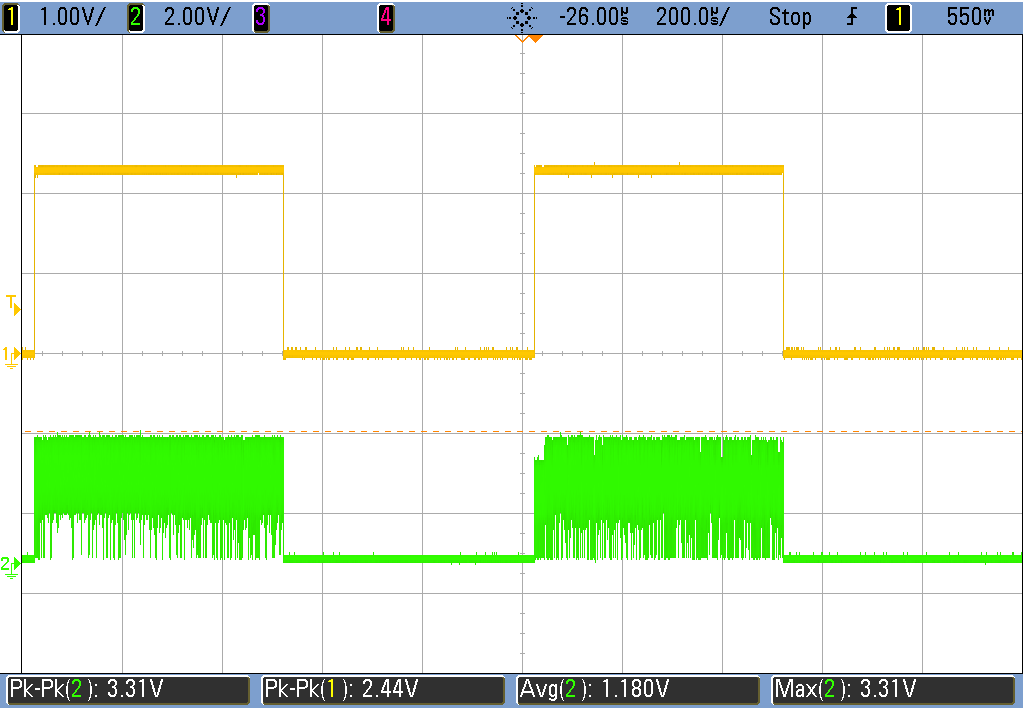
\includegraphics[scale=0.19]{HC-LS-2p3V.png}
        \caption{\color{cyan}74HC02 load to 74LS02}
        \label{fig:ej2exhctols}
    \end{figure}

The reason for this variation in CMOS could be explain by the high impedance at the input making the floating pin induce electric current by noise, creating random values to the output. For this reason, it is recommended in the data-sheet to connect the floating input to the GND or to Vcc depending to the situation, so that unexpected variations wouldn't affect the measurements.

\subsection{\color{purple}TTL loaded to CMOS}

Having the TTL loaded to CMOS as the following figure, with a input value being a quadratic function. 

\begin{figure}[h!]
        \centering
        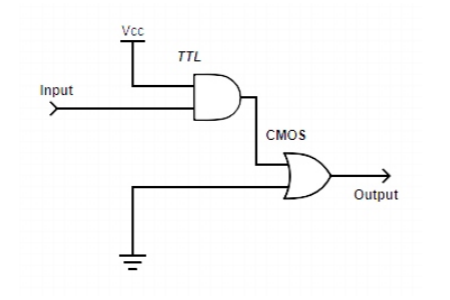
\includegraphics[scale=0.6]{../Exercise5/cir5.png}
        \caption{\color{cyan}TTL loaded to CMOS circuit}
        \label{fig:ej5cir}
\end{figure}

\pagebreak

When the TTL output value is a logical 1, a voltage from 2.4 to 5V is generated. But there is a problem within this values because the input values for a 1 in CMOS components is from 3.15 to 5V, so in the range of 2.4 to 3.15V the input value for the CMOS is undefined which may causing problems while measuring the two components loaded.

\begin{figure}[h!]
        \centering
        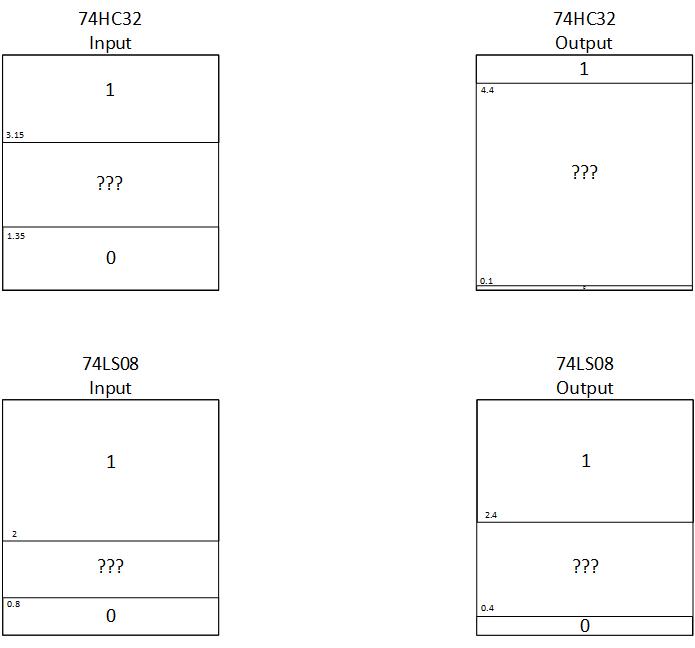
\includegraphics[scale=0.45]{../Exercise5/Graficos5.png}
        \caption{\color{cyan}Theoretical input and output noise margins}
        \label{fig:ej5noisemargin}
\end{figure}

A solution to this problem may be utilizing the same technology components, this is to say using only TTL or CMOS, so that the defined values of the output from the first component is always in range of the input values in the second one. Another solution for this could be utilizing a HCT integrated circuit, a CMOS sub-family, which can make possible the the compatibility between TTL and CMOS by having the following noise margin characteristics. 

\begin{figure}[h!]
        \centering
        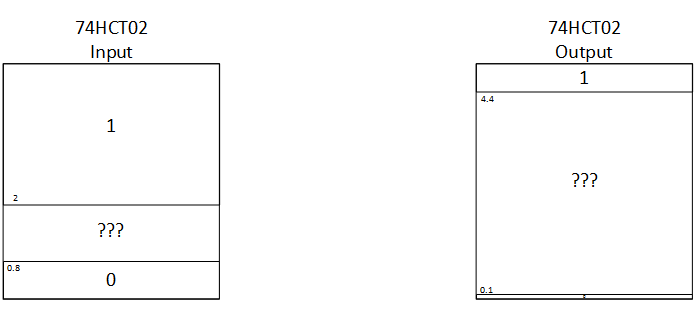
\includegraphics[scale=0.45]{../Exercise5/dataaa5.png}
        \caption{\color{cyan}HCT noise margins}
        \label{fig:ej5noisemargin}
\end{figure}


%\end{document}
\input{../Exercise6/latex/Ex6.tex}
\input{../Exercise7/latex/Ex7.tex}
\pagebreak
\section{\color{olive}Exercise 8}

In this section we will explain how we developed the PCB that made
the sensor HC-SR04 work using only digital electronics. 

\begin{figure}[h!]
\begin{centering}
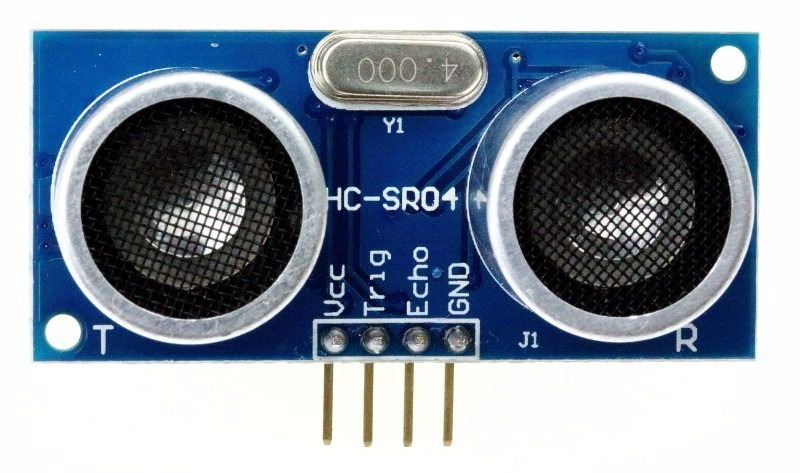
\includegraphics[scale=0.2]{../Exercise8/Informe/images/HC-SR04}
\par\end{centering}
\caption{\color{cyan}Sensor HC-SR04}
\end{figure}

First of all we have to explain how that sensor works.

\subsection{\color{purple}Sensor Operation}

This sensor has 4 pins, 2 for supply voltage (VCC and GND), and another
pair for control, these are 'Trig' and 'Echo'. The operation of this
sensor is pretty simple, you have to send a pulse of time greater
than $10\mu S$ and after some time, it will return into pin Echo,
a response pulse of duration that we will call \emph{T}. If we find
a method to measure the time \emph{T}, we can calculate the distance
measured with the following formula.

\[
Distance=\frac{T}{58}
\]

Its important to know that the time \emph{T }has to be in units of
$\mu S$ for the formula to work properly, and \emph{Distance }is
in centimeters.

A diagram of this can be found in Figure \ref{8_2}

\begin{figure}[h!]
\begin{centering}
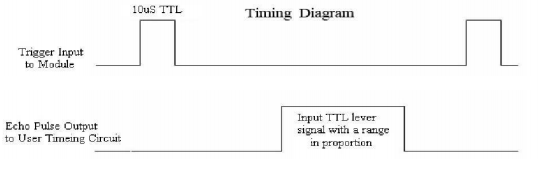
\includegraphics[scale=0.7]{../Exercise8/Informe/images/SENSOR_DIAGRAM}
\par\end{centering}
\caption{\color{cyan}Sensor Input and output}
\label{8_2}

\end{figure}

\subsection{\color{purple}Components used for this Printed Circuit Board}

For this development we utilized the following Integrated Circuits
and components:
\begin{itemize}
\item 74HC4040 Counter 
\item 74HC74 D-type flip-flop
\item Two 74HC00 NAND gates
\item Two NE555 Precision Timers
\item Seven Capacitors
\item Sixteen Resistors
\item Two Diodes
\item Eight Light Emitting Diodes
\end{itemize}
The disposition of this elements in the PCB will be explained as we
undertand how we made this work.

\subsection{\color{purple}PCB Operation}

To make this happen, we develop this board that roughly operates as
shown in Figure \ref{8_3}

\begin{figure}[h!]
\begin{centering}
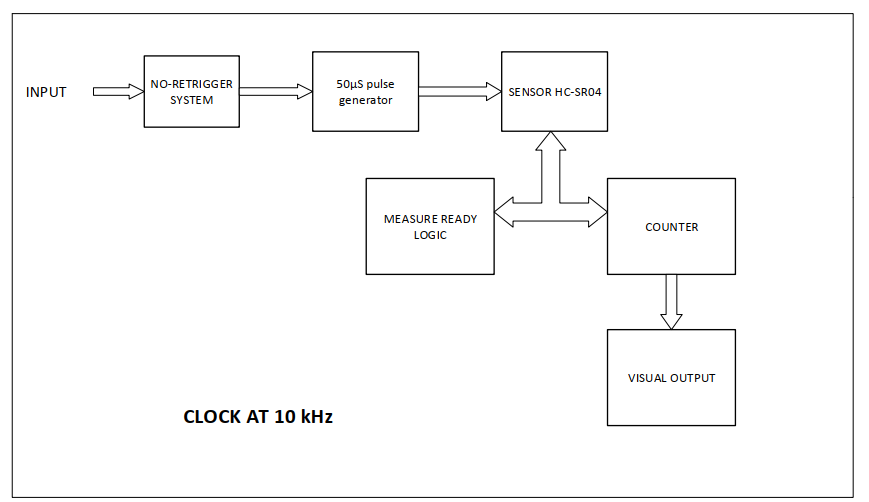
\includegraphics[scale=0.5]{../Exercise8/Informe/images/Diagrama_a_gran_escala}
\par\end{centering}
\caption{\color{cyan}PCB diagram}

\label{8_3}
\end{figure}

First, we have a No-Retrigger System (NRS) that filters all the retriggered
pulses we have because of buttons, that can make our board function
in an unnapropiate way. Then we generate a $50\mu S$ pulse with the
pulse generator, to send to the Trig pin of the sensor. Once we have
the respone of the sensor, we connect the Echo pin with the counter
and the measure ready logic. And finally, we plug a visual output
to the counter to see the measurement we have made. Every module seen
on this diagram, is powered by a $10kHz$ clock.

\subsubsection{\color{red}No-Retrigger System operation}

This system is powered by a 74HC74 D-type flip flop that with the
proper connections we've changed it to an asynchronous SR Flip-Flop(SRFF).
To make this, we connected the SRFF pins as follows:

\begin{figure}[h!]
\begin{centering}
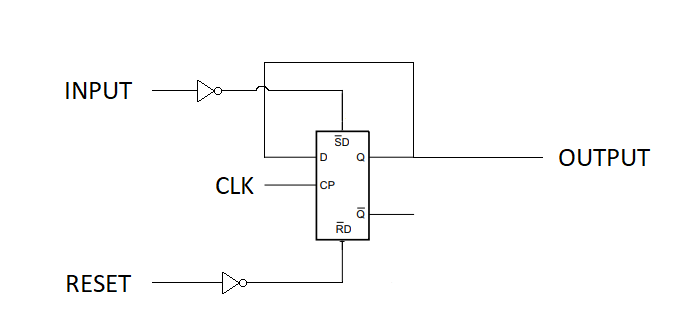
\includegraphics[scale=0.5]{../Exercise8/Informe/images/NO-RETRIGGER_SYSTEM}
\par\end{centering}
\caption{\color{cyan}No-Retrigger System Connections}

\end{figure}

By making this connections we made a feedback with the Q and D pins
so by every positive-edge clock Q is maintained to its previous value,
unless RESET is on. So, summarizing, by connecting the INPUT pin to
the input button, and the RESET pin to the reset button, we've created
a No-Retrigger System for our board.

\subsubsection{\color{red}50 Microseconds Pulse Generator}

Making this pulse generator was a challenge, but we achieved it by
creating two submodules into the $50\mu S$ Pulse Generator Module,
these are the differentiator circuit, and the pulse generator circuit.
Tough the Differentiator Circuit is placed before the Pulse Generator
Circuit (PGC), we will explain first the PGC to better understand
the utility of the Differentiator.

\paragraph{Pulse Generator Circuit}

To power this pulse generator we've used a NE555 Precision Timer,
that by connecting it as shown in Figure \ref{8_5}, we have made
a Pulse generator of the timme we wanted.

The formula to obtain the Pulse time at the output is the following

\[
T=ln(3)C3.R2
\]

But there is a problem, this pulse generator only works if the input
pulse time is less than the time calculated on the previous formula.
So if we have a pulse generated by a human that is oviously greater
than $50\mu S$ we need a way to make this still work. So here is
were the Differentiator Circuit comes to help.

\paragraph{Differentiator Circuit}

This circuit basically differentiates an input, for us, this means
that whenever a pulse its made, a set of dirac's deltas comes out
of the circuit, one positive, and another negative. If we define $\tau$
as 

\[
\tau=RC
\]
 and we choose the apropiate values to the resistor and capacitor
to make $5\tau\leq50\mu S$ we can have a really good differentiator
circuit that for every input pulse, it creates an output of less than
$50\mu S$, and we can make work our Pulse Generator.

\begin{figure}[h!]
\begin{centering}
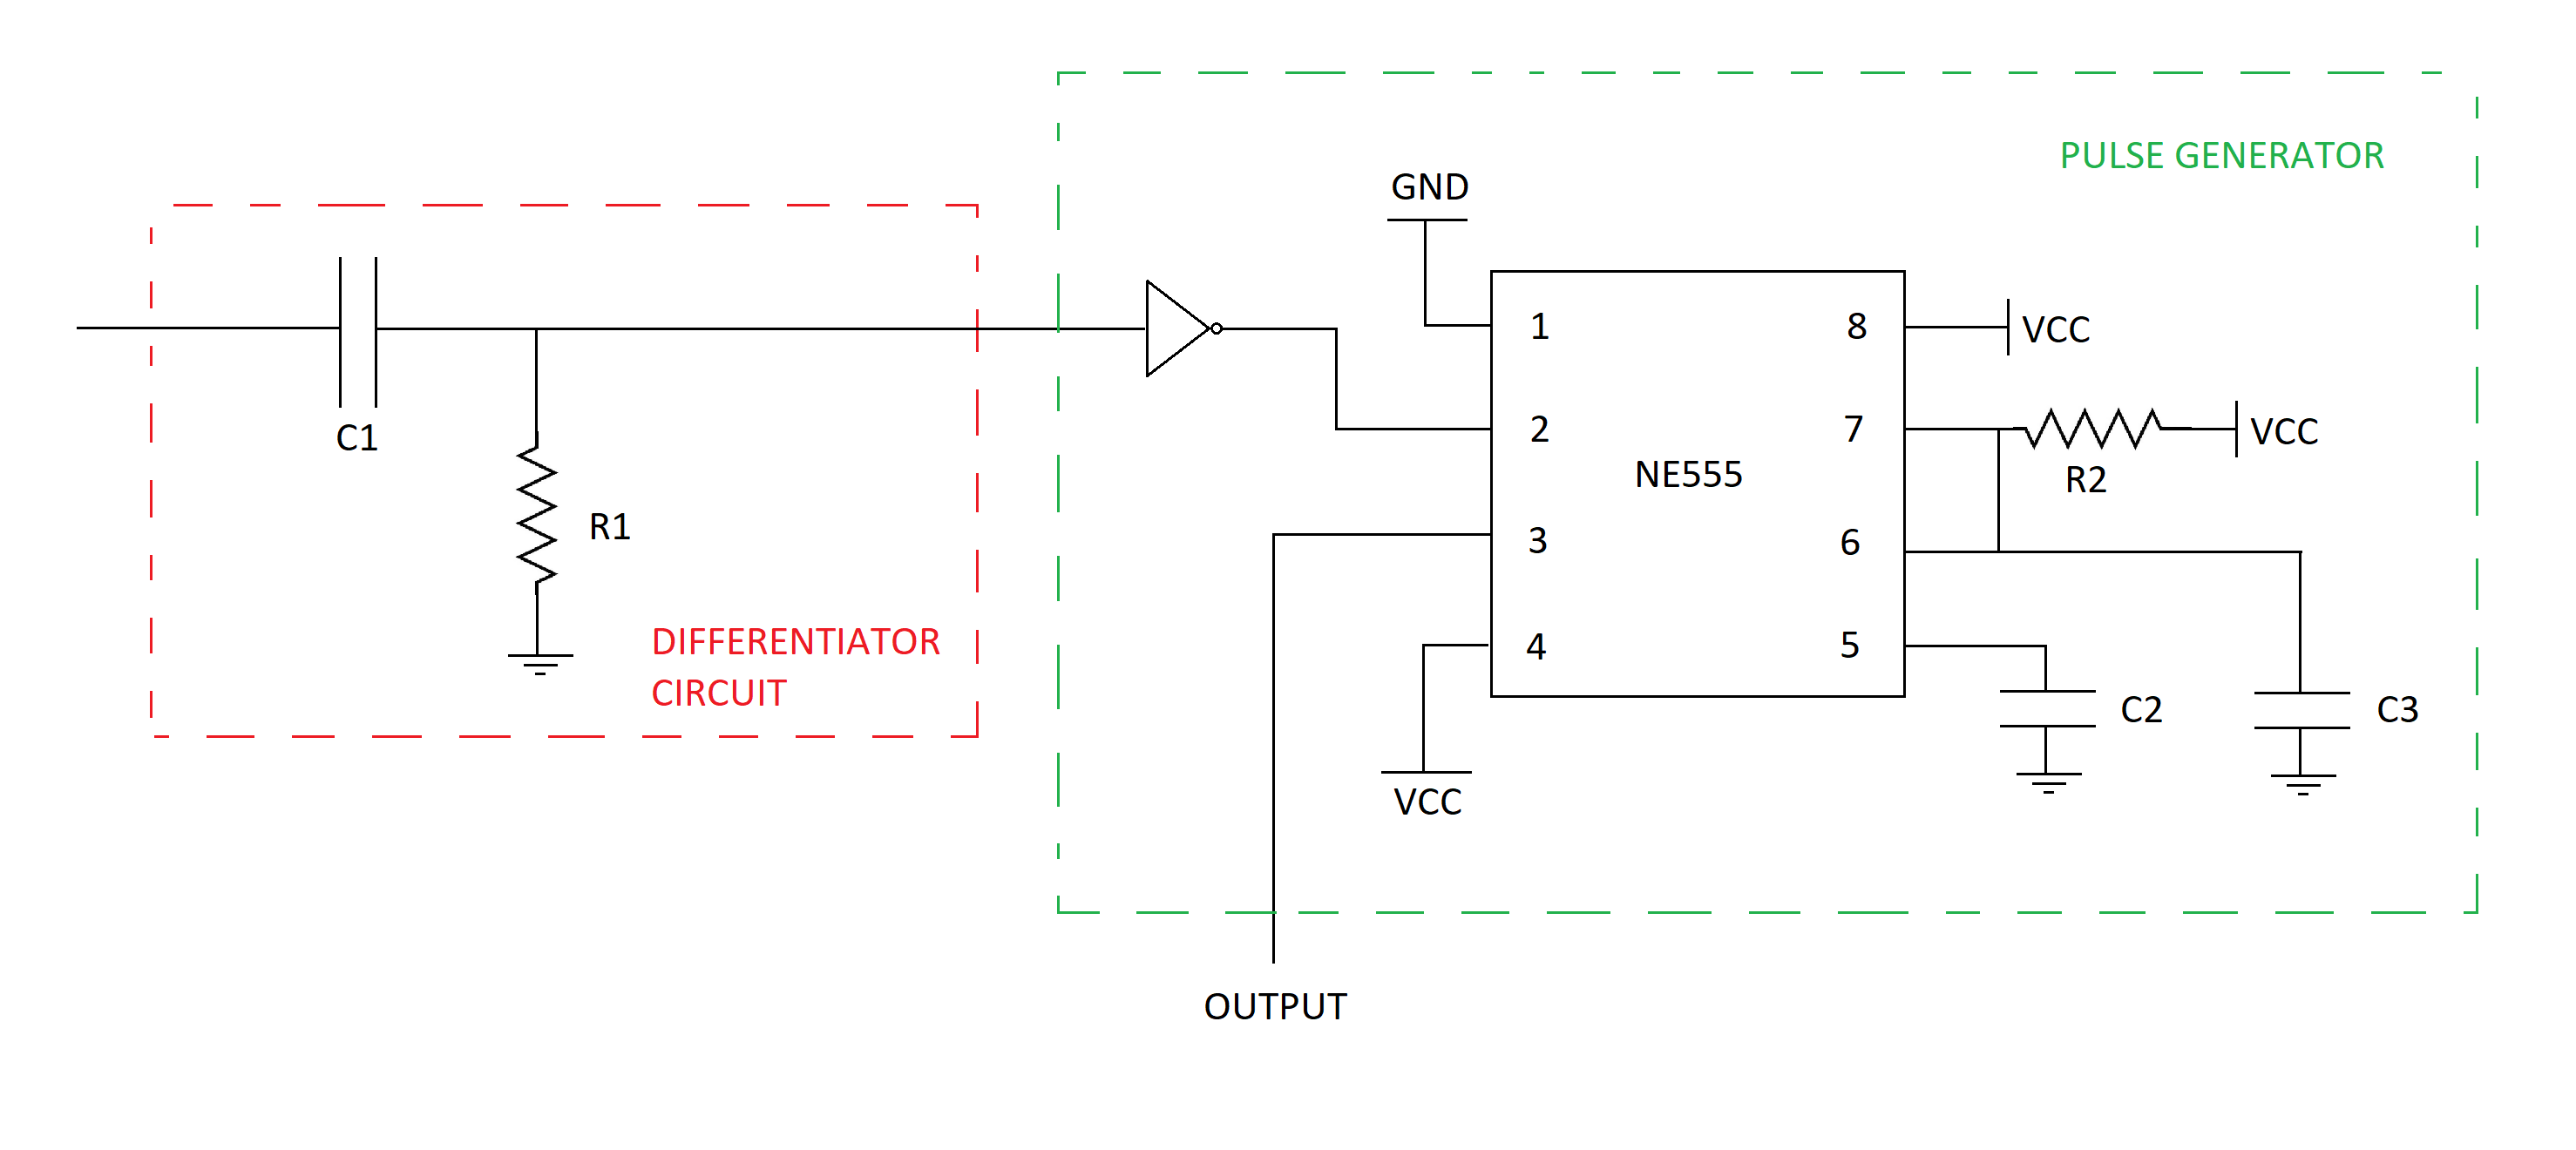
\includegraphics[scale=0.2]{../Exercise8/Informe/images/PULSE_GENERATOR}
\par\end{centering}
\caption{\color{cyan}Pulse Generator}
\label{8_5}
\end{figure}

\subsubsection{\color{red}Measure Ready Logic}

The measure ready logic is powered by a 74HC74 D-type flip flop used
equally as the No-Retrigges System, and a differentiator circuit almost
as equal as the Pulse generator differentiator circuit. But it has
one little difference, the 74HC74 is very sensitive to negative voltage,
and it can stop working properly according to its datasheet, so we
had to add a little protection to erase the negative delta provided
by the differentiator circuit. We made this by simply adding a diode
that cancels that delta. So the circuit became as shown in the Figure
\ref{8_6}

\begin{figure}[h!]
\begin{centering}
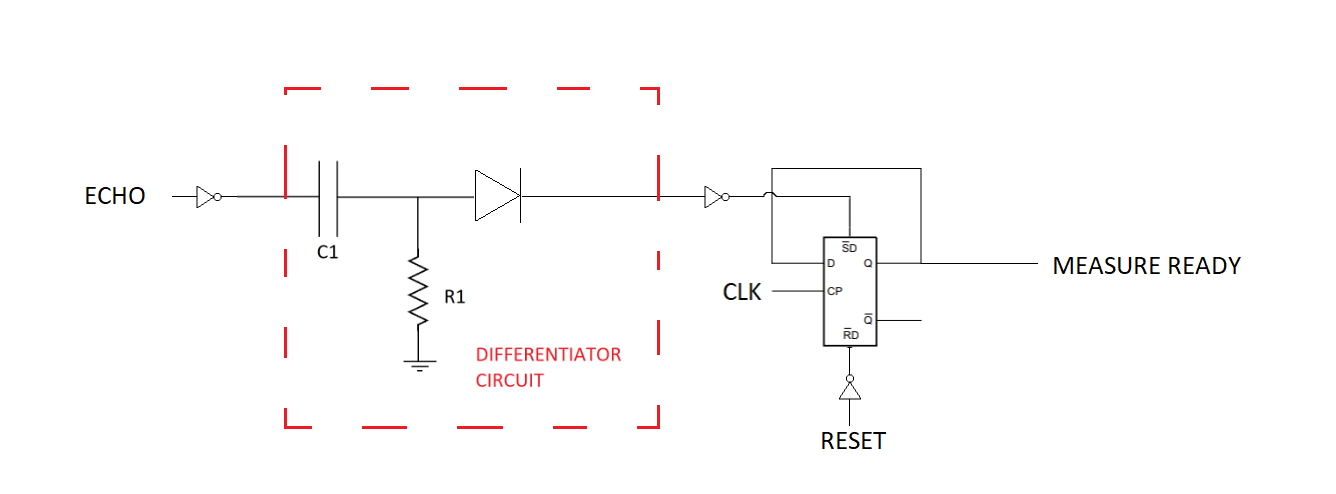
\includegraphics[scale=0.5]{../Exercise8/Informe/images/MEASURE_READY}
\par\end{centering}
\caption{\color{cyan}Measure Ready Logic}

\label{8_6}
\end{figure}

\subsubsection{\color{red}Counter}

This circuit was relatively easy since we used a 74HC4040 Counter
that was really intuitive to use, it was connected as shown in Figure
\ref{8_7}

\begin{figure}[h!]
\begin{centering}
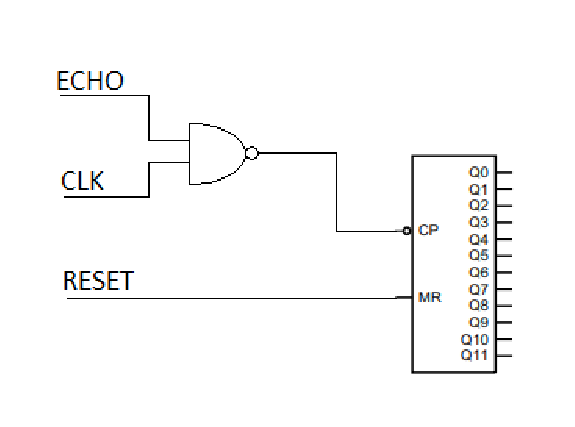
\includegraphics[scale=0.7]{../Exercise8/Informe/images/COUNTER}
\par\end{centering}
\caption{\color{cyan}Counter}
\label{8_7}

\end{figure}

We implemented the NAND before the CP pin to count only when the Echo
is on, and when it becomes off, the counter will stop counting.

\subsubsection{\color{red}Clock}

The clock was performed also with a NE555 and by following the equation

\[
f=\frac{1}{T}=\frac{1.44}{(R2+2.R1).C3}
\]

we made a clock of the period needed. However, due to the resistor
and capacitor values we had on the university, we only achieved a
\emph{T} of roughly of $80\mu S$ instead of the $100\mu S$ we wanted.
Since it made no such big difference, we left it that way.

\begin{figure}[h!]
\begin{centering}
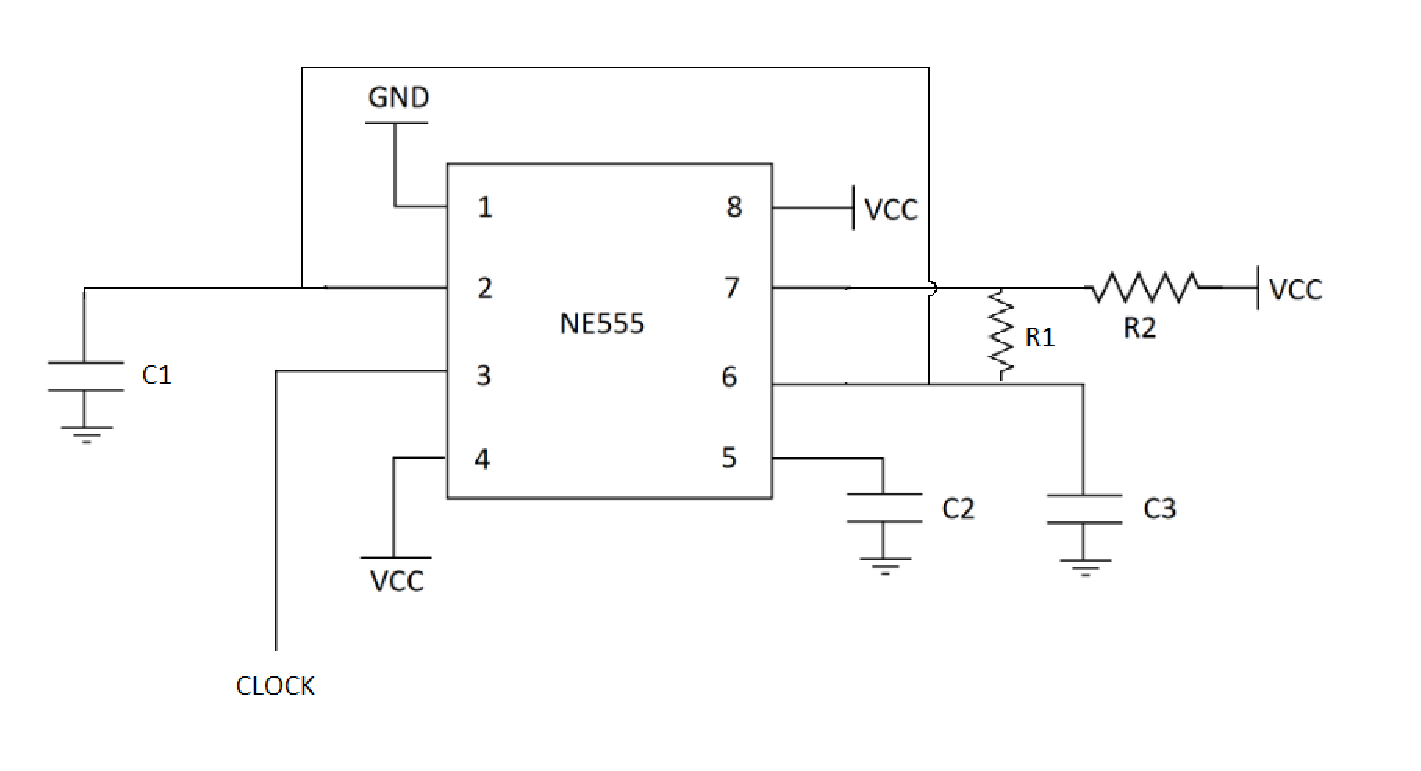
\includegraphics[scale=0.5]{../Exercise8/Informe/images/CLOCK}
\par\end{centering}
\caption{\color{cyan}Clock}

\label{8_8}

\end{figure}

\paragraph{Visual Output}

Finally for this module, we decided to insert a simple array of LEDs
displaying in binary code the measurement made by the sensor.

\subsection{\color{purple}PCB Fabrication}

To fabricate the design explained before, we used Altium 18 to create
the schematic and design the PCB. Because of the amount of things
taken into account explained before, we decided to implement a double
layer PCB, to make this solution fit in an respectable size. Using
the default library provided by Altium and the LIBEBAL library, we
created the design shown on Figure \ref{8_9}

\begin{figure}[h!]
\begin{centering}
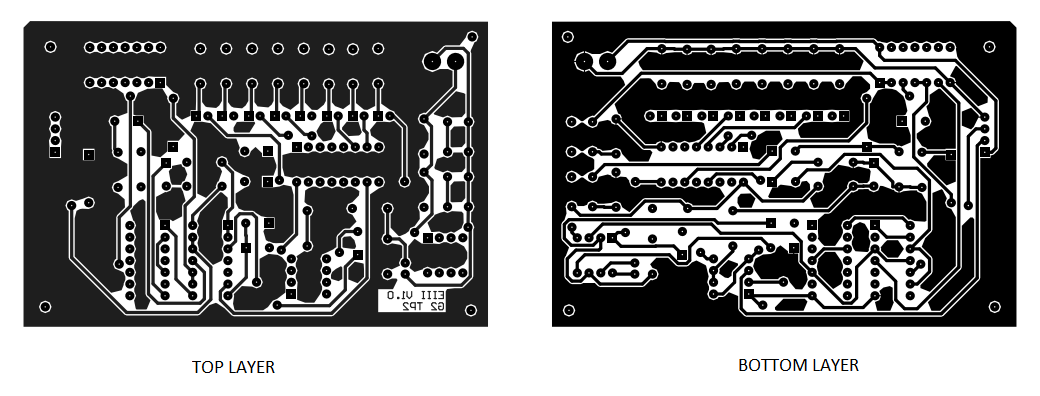
\includegraphics[scale=0.7]{../Exercise8/Informe/images/PCB_Layers}
\par\end{centering}
\caption{\color{cyan}PCB Design}
\label{8_9}
\end{figure}

\begin{figure}[h!]
\begin{centering}
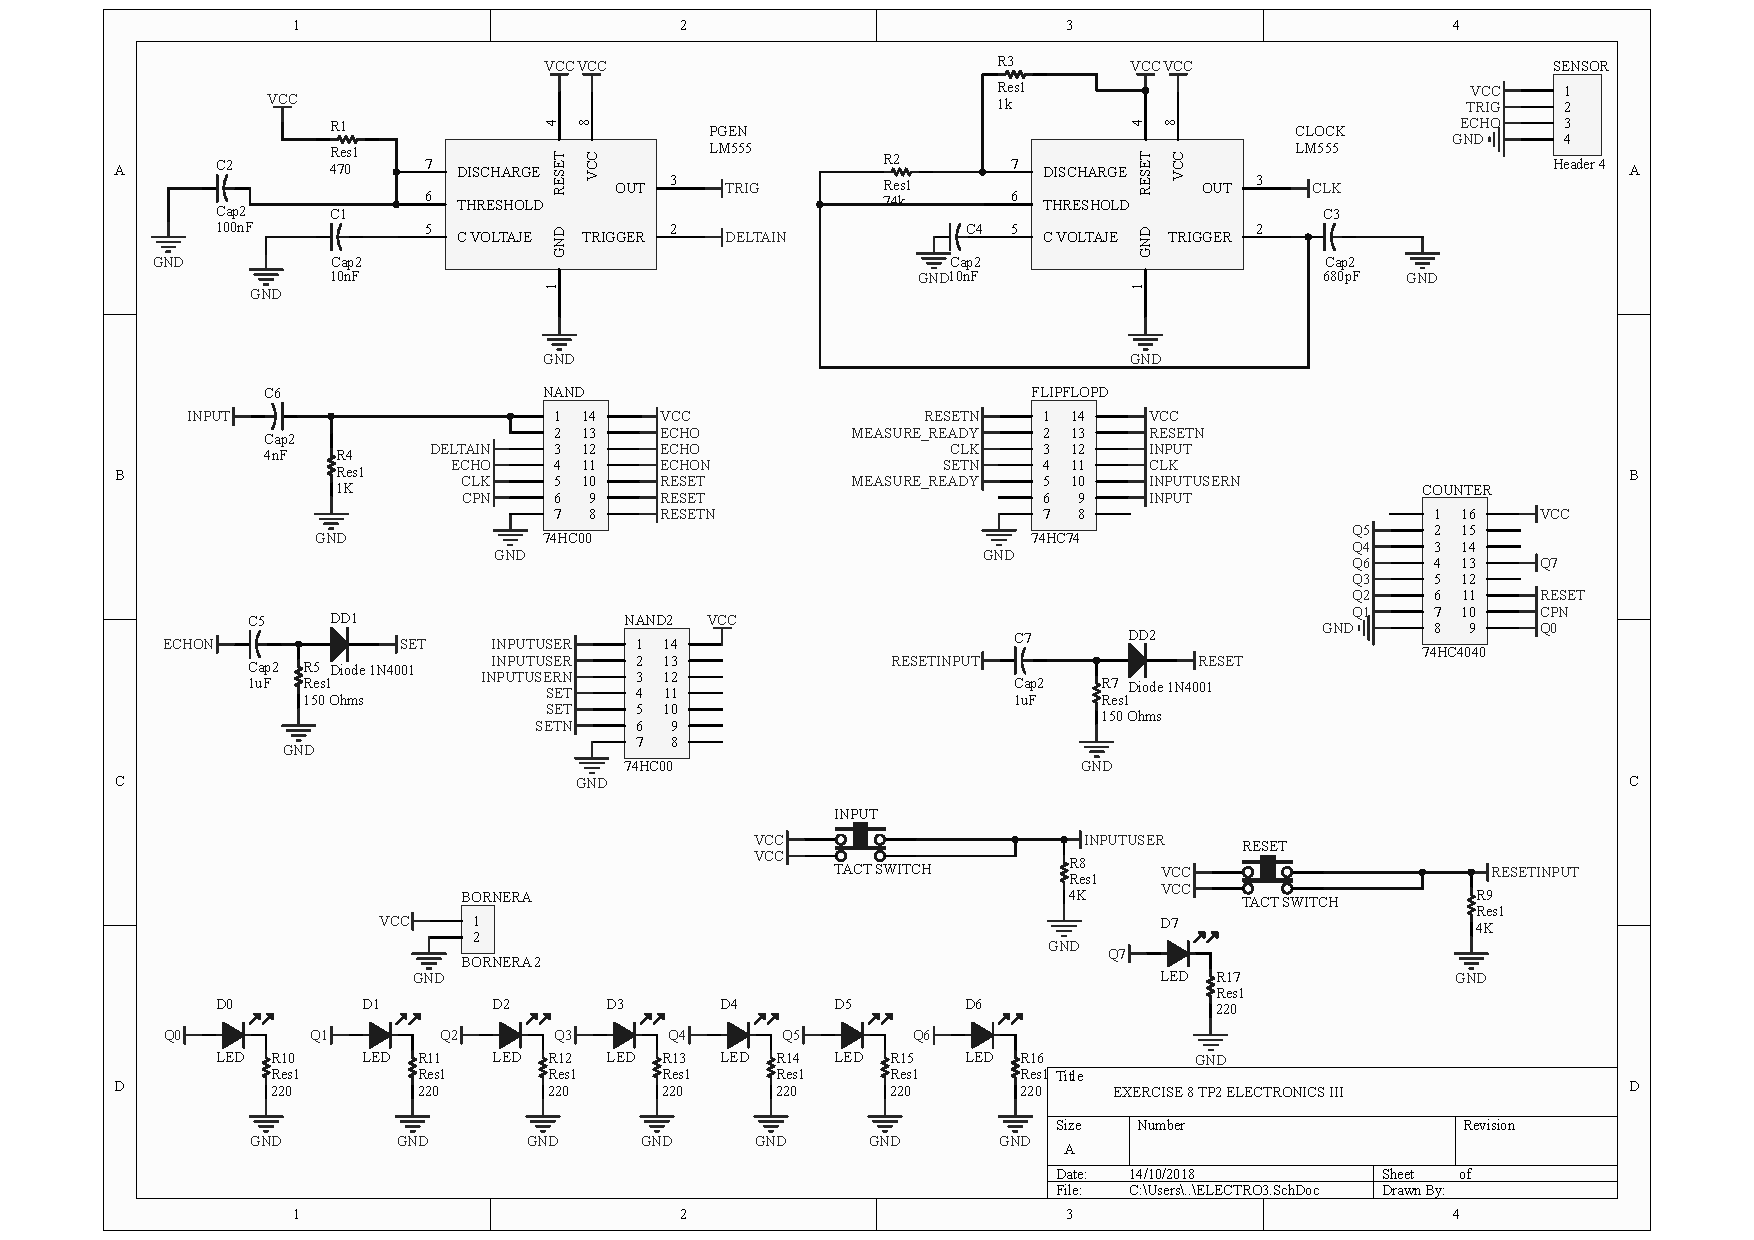
\includegraphics[scale=0.6]{../Exercise8/Informe/Schematic}
\par\end{centering}
\caption{PCB Schematic}

\end{figure}

\begin{figure}[h!]
\begin{centering}
\includegraphics[scale=0.05]{../Exercise8/Informe/images/TOP} 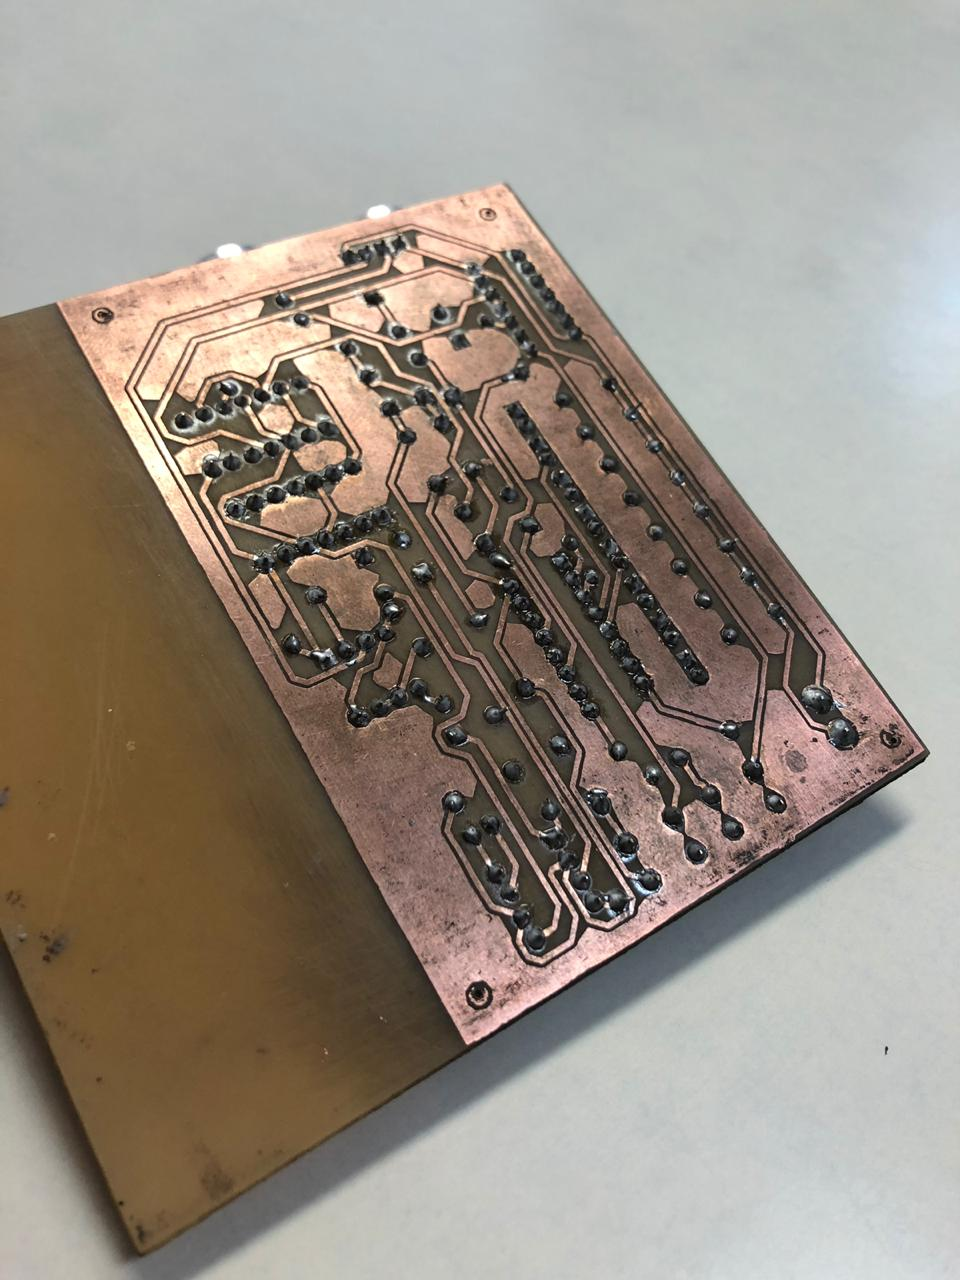
\includegraphics[scale=0.16]{../Exercise8/Informe/images/BOT}
\par\end{centering}
\caption{\color{cyan}PCB Top and Bottom Layer}

\end{figure}

\subsection{\color{purple}Ussage}

To use this solution one simply has to connect the Board to 5V voltage
tension, and press the reset button. Once you are ready to measure,
press the Input Button and a measurement in binary code will be displayed
in the LEDs placed in the PCB. If we call \emph{n} the number in decimal
obtained by the LEDs, we obtain the measurement by following the next
equation

\[
Distance=\frac{n.80}{58}(cm)
\]

Where the number 80 comes from the clock speed and the 58 from the
formula given from the sensor.

\subsection{\color{purple}Simulation}

For the simulation a counter with the logic shown on Figure \ref{8_7}
and the clock of Figure \ref{8_8} was made. This was accomplished
by writeng hardware descriptive code on verilo and simulated on GTK
wave. The results were as shown on Figure \ref{8_13}.

\begin{figure}[h!]
\begin{centering}
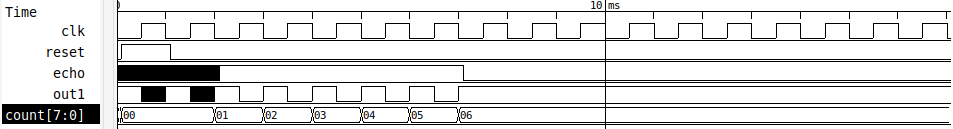
\includegraphics[scale=0.5]{../Exercise8/Informe/images/Count_simulation}
\par\end{centering}
\caption{\color{cyan}Verilog Simulation}
\label{8_13}

\end{figure}

As we've seen, the circuits make what we were expecting, so we conclude
that everyting should work ok on the real implementation.

\subsection{\color{purple}Conclusions}

We conclude that the Board behaves as expected, and by adjusting the
formula with 80, we can obtain a relatively great measurement of the
distance. Because fabrication and design limitations, we decided not
to add the measure ready LED to display that. This was because to
human perspective, the measurement is practically instant and adding
2 more components to the PCB was not enough gain to make the trouble.
However, the Board to our perspective works perfectly.


%\newpage
\pagenumbering{roman}
\section{Appendix}

\begin{figure}[h!] %cambio la H por!
\begin{centering}
\includegraphics[scale=0.4]{../E4TP1/images/5}
\par\end{centering}
\caption{\color{cyan}Verilog implementation of Excercise 4}
\label{fig:figura4.6}
\end{figure}

\begin{figure}[h!]%cambio la H por!
\begin{centering}
\includegraphics[scale=0.4]{../E4TP1/images/6}
\par\end{centering}
\caption{\color{cyan}Terminal's output of Excercise 4}
\label{fig:figura4.7}
\end{figure}


%%% End document
\end{document}
